\begin{frame}
  \frametitle{Simulation setup}
  \begin{itemize}
  \item[-] emulated Kuka FRI Joint specific impedance control mode
    \begin{itemize}
    \item[] $\boldsymbol{\tau}_{cmd} = K_j(\vec{q}_{FRI} - \vec{q}_{msr}) + D(d_{j}) + \boldsymbol{\tau}_{FRI} + \vec{f}_{dynamics}(\vec{q}, \dot{\vec{q}}, \ddot{\vec{q}})$
    \end{itemize}
  \item[-] $K_j = 0$
  \item[-] $\vec{q}_{FRI} = \vec{q}_{msr}$
  \item[-] $d_{j} = 0$
  \item[-] $\vec{f}_{dynamics}(\vec{q}, \dot{\vec{q}}, \ddot{\vec{q}})$ supposed to be $\vec{G}(\vec{q})$ evaluated using KDL library
  \item[-] $\boldsymbol{\tau}_{FRI}$ used as commanded torque
  \item[-] controller @ $1$kHz
  \end{itemize}

\end{frame}

\begin{frame}
  \frametitle{Simulation setup}
  \framesubtitle{Issues}
  \begin{flalign*}
    &\boldsymbol{\tau}_{FRI} = C \dot{\vec{q}} +  B\vec{a}_{app}(\vec{\dot{q}})\\
    &\boldsymbol{\tau}_{FRI} = C \dot{\vec{q}} + J^{T}_{F} ( B_A \vec{a}_{hic}(\vec{w}_{F}, \dot{\vec{q}}) - B_A \dot{J_{A,E}} \vec{\dot{q}} + \vec{w}_{F}) + \boldsymbol{\tau}_{null}(J_{a_{4}})
  \end{flalign*}
  
  \begin{itemize}
  \item[-] $B$ given by KDL {\color{dgreen}\cmark}
  \item[-] $C \dot{\vec{q}}$ given by KDL {\color{dgreen}\cmark}
    
  \item[-] only $\vec{q}$ is available (as in the real scenario)
    \begin{itemize}
    \item[-] $\dot{\vec{q}}$ estimated using an exponential smoothing {\color{orange}\cmark}
    \end{itemize}
    
  \item[-] Jacobians are evalutated using KDL library {\color{dgreen}\cmark} 

    \item[-] $\vec{w}_F$ given by force/torque sensor plugin (software)
      \begin{itemize}
      \item[-] corrupted signal when the tool is mounted on the wrist $\longrightarrow$ massless tool{\color{orange}\cmark}
    \end{itemize}
    \item[-] joints friction and contact friction neglected for ease of simulation {\color{orange}\cmark}
  \end{itemize}
\end{frame}

\begin{frame}
  \frametitle{Simulation setup}
  \framesubtitle{Approaching phase}
  \begin{itemize}
  \item[-] initial configuration: $\begin{bmatrix} -0.71 & 1.15 & 0.39 & 0.52 & -0.54 & -1.57 \end{bmatrix}$
  \item[-] final configuration: $\begin{bmatrix} 0.00 & -0.14 & 0.10 & 0.00 & 3.14 & 0.00 \end{bmatrix}$
  \item[-] duration $5$s
  \item[-] $K_p = \mathrm{diag}(30)$
  \item[-] $K_d = \mathrm{diag}(30)$
  \end{itemize}
\end{frame}

\begin{frame}
  \frametitle{Simulation setup}
  \framesubtitle{Approaching phase - Results}
  \begin{center}
   \vskip-0.1in
    \begin{tabular}{cc}
      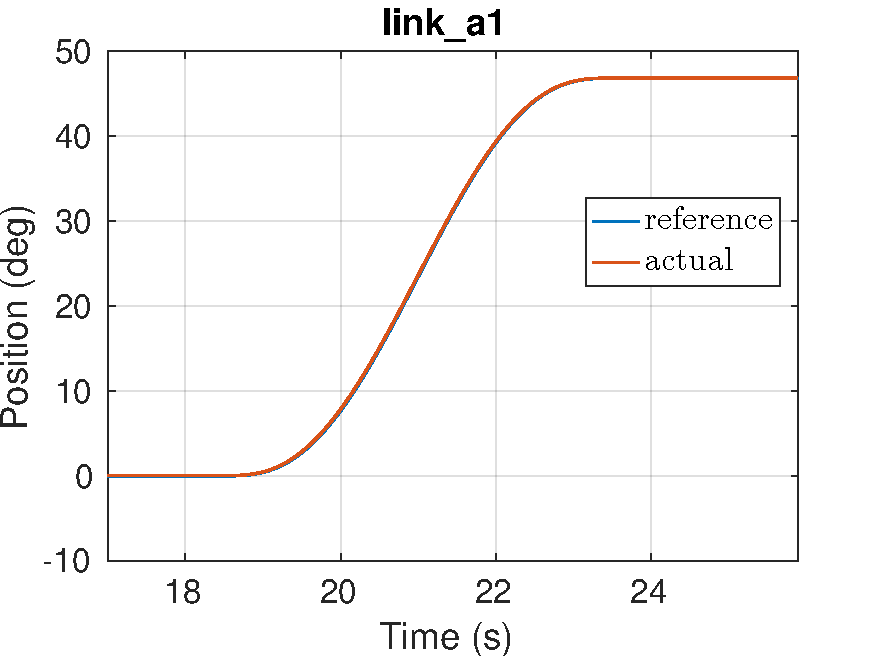
\includegraphics[scale=0.34]{cart_sim_a1} &
      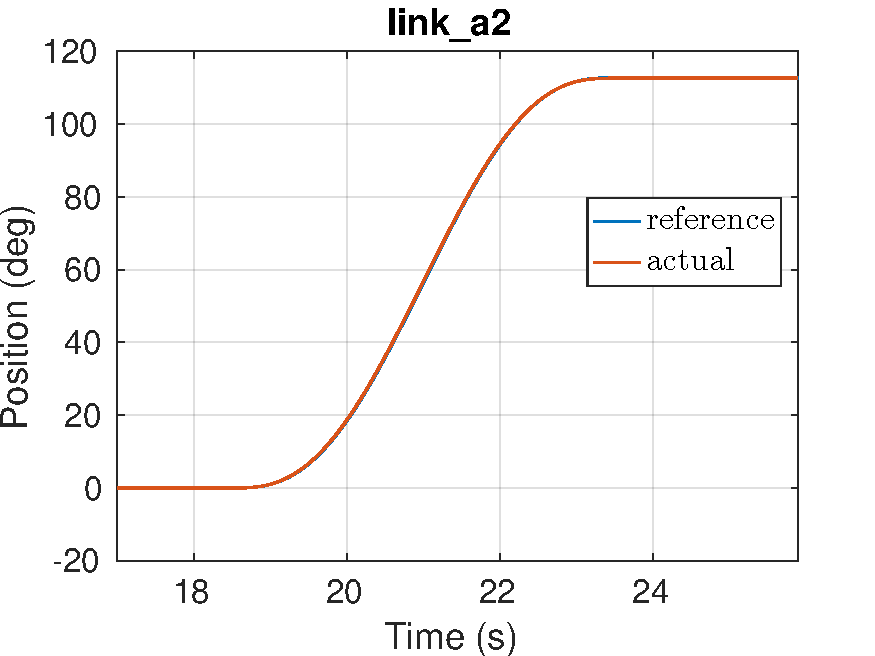
\includegraphics[scale=0.34]{cart_sim_a2}
    \end{tabular}
  \end{center}
  \begin{center}
   \vskip-0.1in
    \begin{tabular}{cc}
      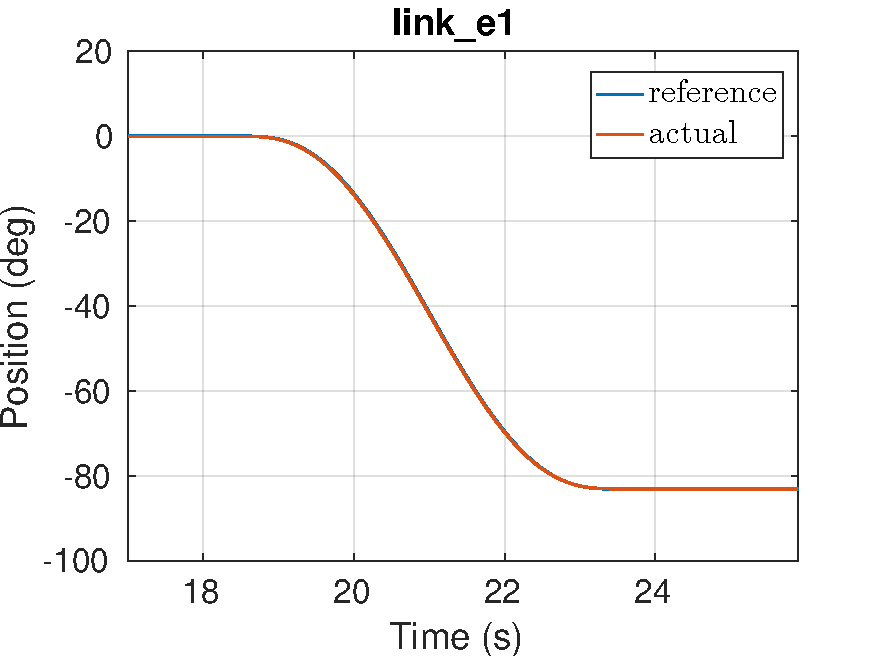
\includegraphics[scale=0.34]{cart_sim_e1} &
      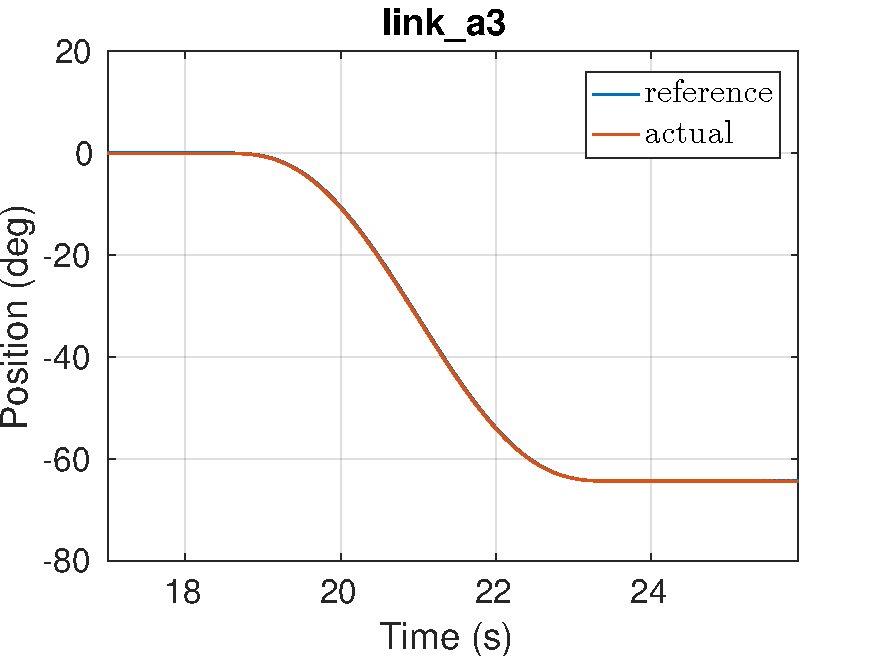
\includegraphics[scale=0.34]{cart_sim_a3}
    \end{tabular}
  \end{center}
\end{frame}

\begin{frame}
  \frametitle{Simulation setup}
  \framesubtitle{Approaching phase - Results}
  \begin{center}
   \vskip-0.1in
    \begin{tabular}{cc}
      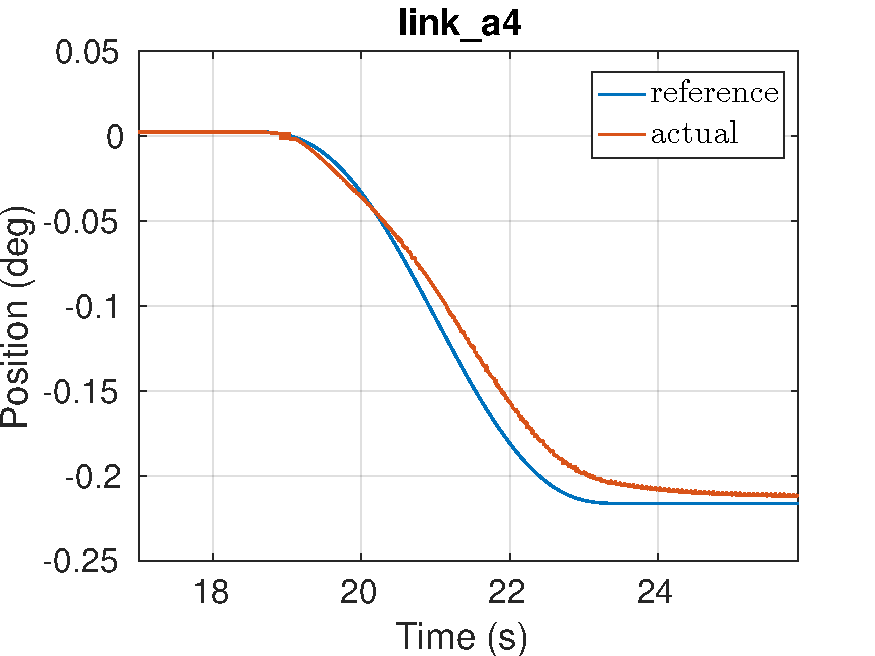
\includegraphics[scale=0.34]{cart_sim_a4} &
      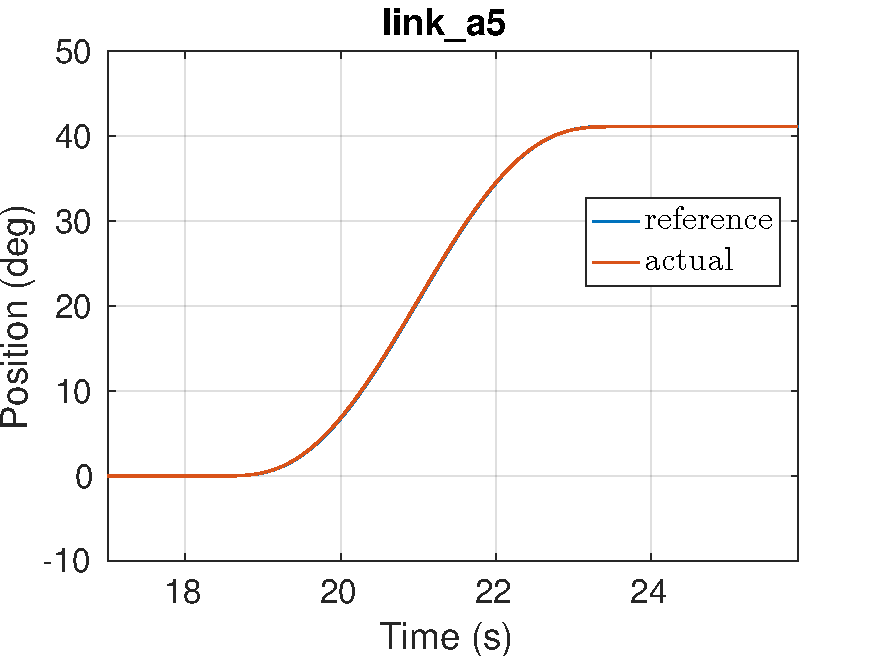
\includegraphics[scale=0.34]{cart_sim_a5}
    \end{tabular}
  \end{center}
  \begin{center}
   \vskip-0.1in
    \begin{tabular}{c}
      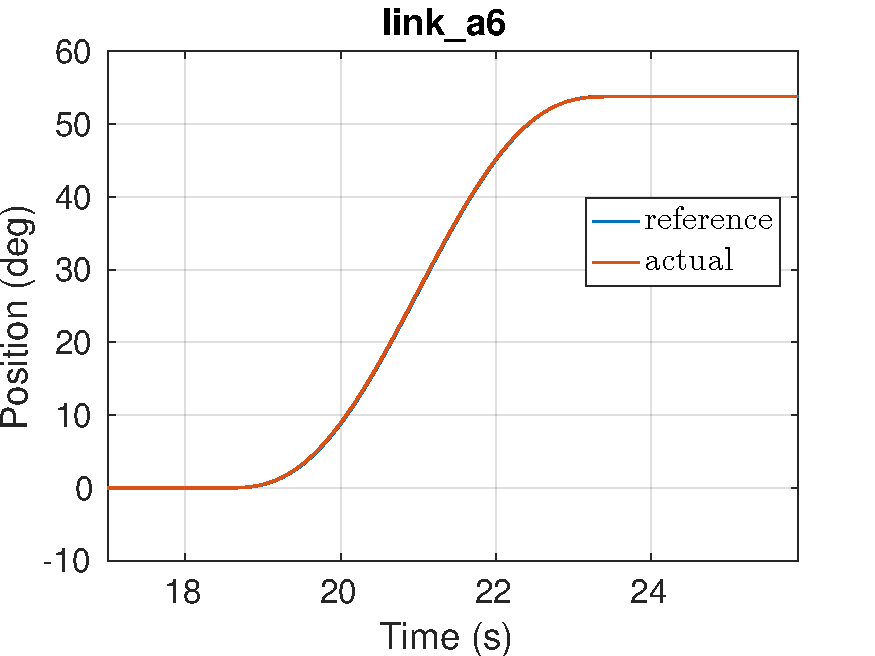
\includegraphics[scale=0.34]{cart_sim_a6}
    \end{tabular}
  \end{center}
\end{frame}

\begin{frame}
  \frametitle{Simulation setup}
  \framesubtitle{Force regulation}
  \begin{itemize}
  \item[-] duration $2$s
  \item[-] $K_p = \mathrm{diag}(30)$
  \item[-] $K_d = \mathrm{diag}(30)$
  \item[-] $k_{f} = 2$
  \item[-] $b_f = 25$
  \end{itemize}
\end{frame}

\begin{frame}
  \frametitle{Simulation setup}
  \framesubtitle{Force regulation- Results}
  \begin{center}
   \vskip-0.1in
    \begin{tabular}{cc}
      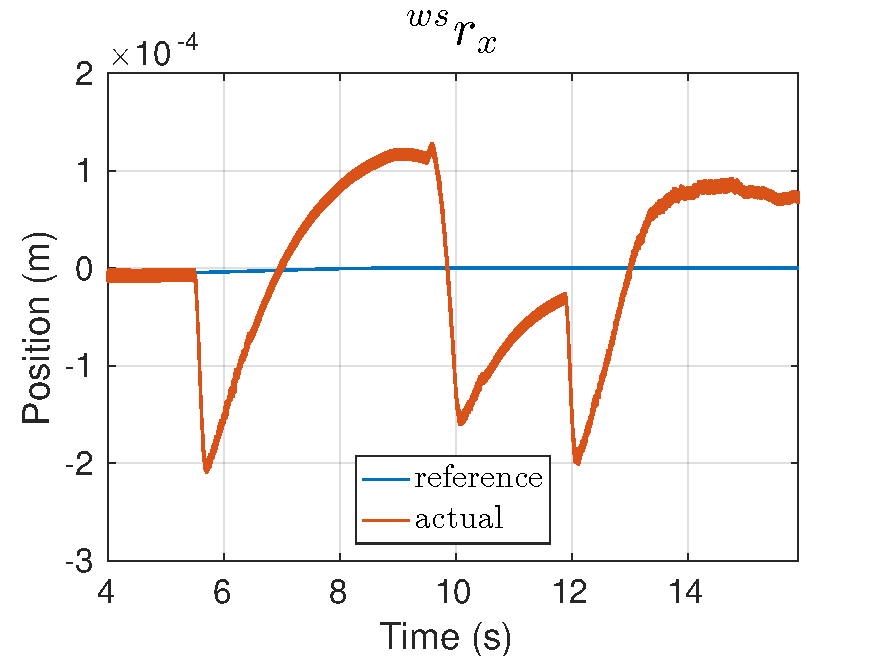
\includegraphics[scale=0.34]{force_sim_1_x} &
      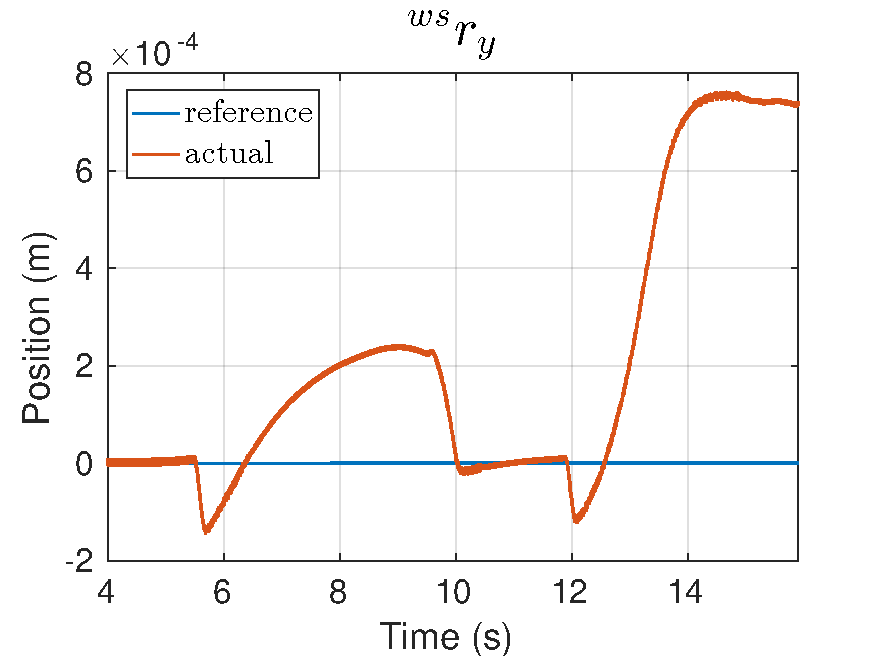
\includegraphics[scale=0.34]{force_sim_1_y}
    \end{tabular}
  \end{center}
  \begin{center}
   \vskip-0.1in
    \begin{tabular}{c}
      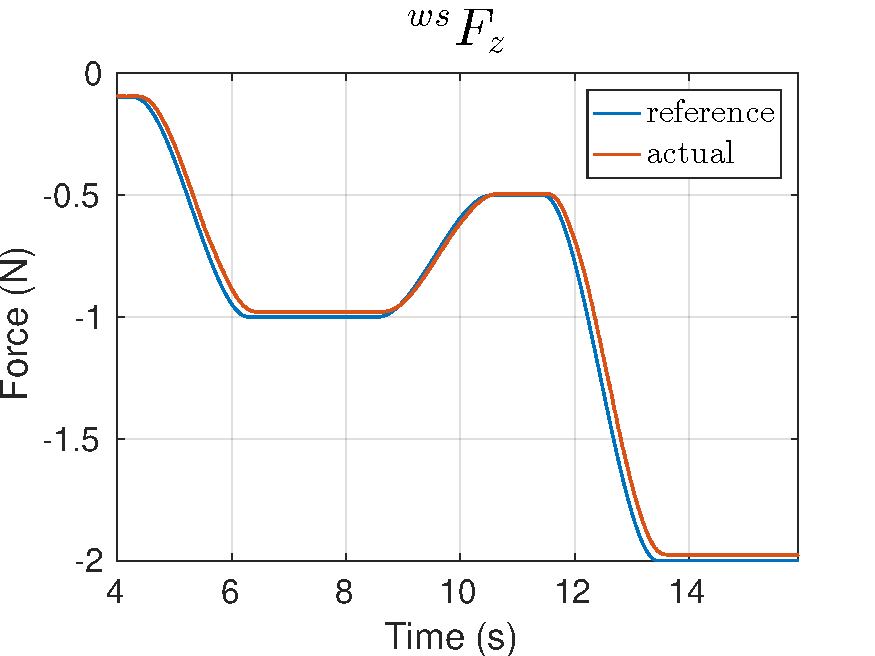
\includegraphics[scale=0.34]{force_sim_1_z}
    \end{tabular}
  \end{center}
\end{frame}

\begin{frame}
  \frametitle{Simulation setup}
  \framesubtitle{Force regulation + motion}
  \begin{itemize}
  \item[-] reference trajectory duration $5$s
  \item[-] reference force duration $2$s
  \item[-] $K_p = \mathrm{diag}(30)$
  \item[-] $K_d = \mathrm{diag}(30)$
  \item[-] $k_{f} = 2$
  \item[-] $b_f = 25$
  \end{itemize}
\end{frame}

\begin{frame}
  \frametitle{Simulation setup}
  \framesubtitle{Force regulation + motion - Results}
  \begin{center}
   \vskip-0.1in
    \begin{tabular}{cc}
      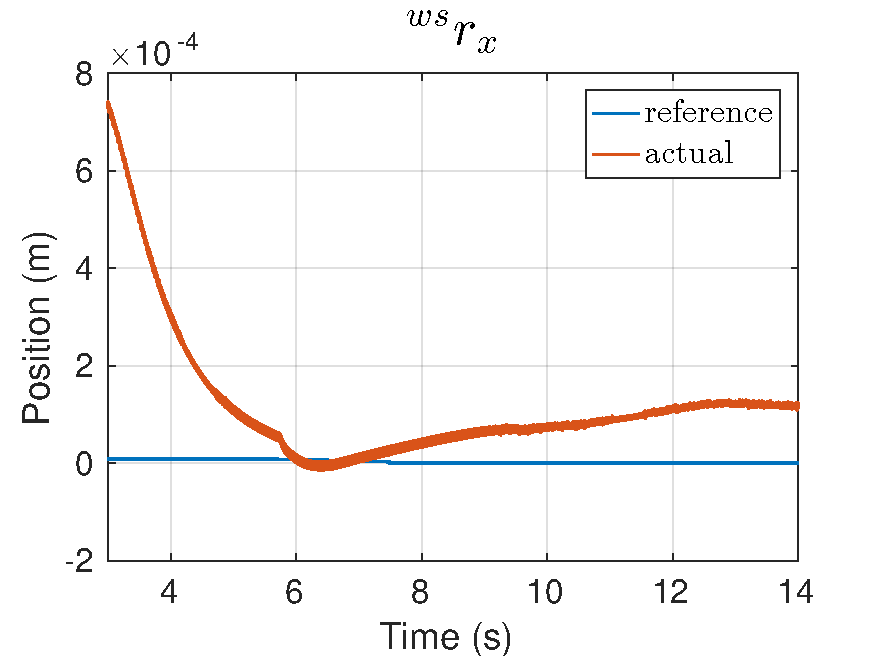
\includegraphics[scale=0.34]{force_sim_2_x} &
      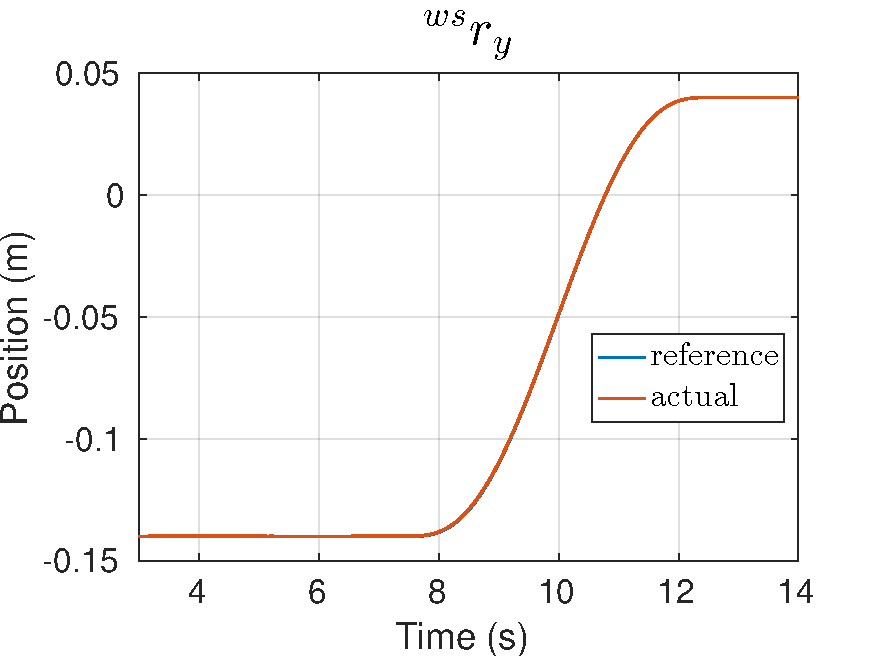
\includegraphics[scale=0.34]{force_sim_2_y}
    \end{tabular}
  \end{center}
  \begin{center}
   \vskip-0.1in
    \begin{tabular}{c}
      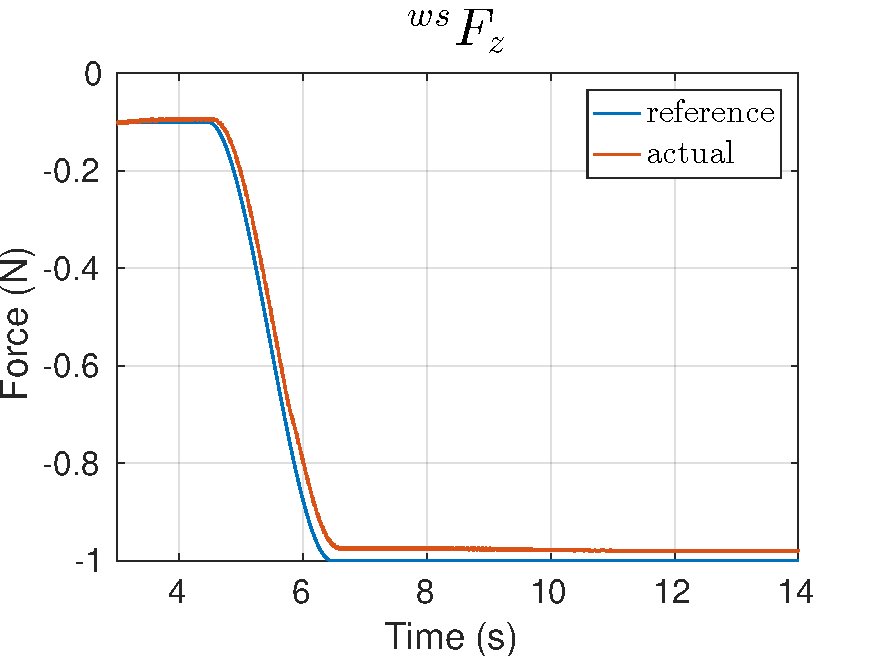
\includegraphics[scale=0.34]{force_sim_2_z}
    \end{tabular}
  \end{center}
\end{frame}
